%=========================================================
% Capítulo 11 — O futuro da assimilação de dados
%=========================================================
\chapter{O futuro da assimilação de dados}
\label{ch:futuro}

\noindent\textbf{Resumo:}
Este capítulo explora as fronteiras emergentes da assimilação de dados (AD), com ênfase na integração entre métodos híbridos, aprendizado de máquina e sistemas acoplados do Sistema Terrestre.
Também são discutidos os desafios específicos da assimilação em regiões tropicais e o papel dos novos sensores na melhoria das condições iniciais e da representação física dos processos atmosféricos.

%---------------------------------------------------------
\section{A evolução contínua da assimilação de dados}
A assimilação de dados evoluiu de simples métodos de interpolação para sofisticados sistemas probabilísticos capazes de fundir bilhões de observações diárias.
Entretanto, mesmo após décadas de avanços, persistem desafios relacionados à complexidade dos modelos, aos erros correlacionados e à representação dos processos não lineares.
O futuro da AD depende de estratégias híbridas, uso de inteligência artificial e uma visão integrada do Sistema Terrestre.

%---------------------------------------------------------
\section{Métodos híbridos e aprendizado de máquina}
Os métodos híbridos representam a síntese entre abordagens variacionais (4DVar) e estatísticas (EnKF).
A próxima geração de sistemas está incorporando componentes baseados em \emph{machine learning} (ML) para resolver limitações persistentes:
\begin{itemize}
  \item aprendizado dinâmico de matrizes de erro de background ($\mathbf{B}$) a partir de ensembles históricos;
  \item redes neurais capazes de estimar operadores de observação ($\mathbf{H}$) e jacobianos aproximados;
  \item correção de erros sistemáticos de modelo por redes de aprendizado residual;
  \item assimilação \emph{end-to-end}, onde o modelo e a assimilação são treinados de forma conjunta.
\end{itemize}

O uso de ML reduz o custo computacional de operadores complexos, especialmente radiativos, e permite explorar informações observacionais ainda subutilizadas.

\begin{figure}[h!]
\centering
\begin{tikzpicture}[>=latex]
  \node[draw,rounded corners,fill=blue!10,minimum width=3cm] (ens) {Ensemble Kalman};
  \node[draw,rounded corners,fill=green!10,right=2cm of ens] (ml) {Rede Neural};
  \node[draw,rounded corners,fill=orange!10,below=1.5cm of $(ens)!0.5!(ml)$] (hibrido) {Método Híbrido};
  \draw[->,thick] (ens) -- (hibrido);
  \draw[->,thick] (ml) -- (hibrido);
\end{tikzpicture}
\caption{Convergência entre assimilação estatística e aprendizado de máquina.}
\label{fig:hibrido-ml}
\end{figure}

Essa convergência não substitui a física do modelo — ela a complementa, permitindo que as técnicas de ML aprendam padrões residuais e não lineares, mantendo o rigor físico.

%---------------------------------------------------------
\section{Assimilação acoplada do Sistema Terrestre}
O avanço da modelagem acoplada (Atmosfera–Oceano–Superfície–Criosfera) trouxe a necessidade de assimilação acoplada — ou \textbf{Earth System Data Assimilation (ESDA)}.
Nessa abordagem, a AD considera as interações entre componentes do sistema:
\begin{itemize}
  \item fluxos de calor, umidade e momentum entre oceano e atmosfera;
  \item acoplamento entre umidade do solo, vegetação e trocas radiativas;
  \item retroalimentação entre gelo marinho, temperatura e circulação global.
\end{itemize}

A assimilação acoplada melhora a coerência entre variáveis e reduz discrepâncias entre subsistemas.
No contexto brasileiro, sistemas como o MONAN incorporam essa filosofia, integrando modelos atmosféricos (MPAS), oceânicos (HYCOM) e de superfície continental (SSiB).

%---------------------------------------------------------
\section{Desafios da assimilação em regiões tropicais}
As regiões tropicais representam um dos maiores desafios da assimilação moderna.
Os sistemas convencionais foram otimizados para latitudes médias, onde as ondas baroclínicas dominam e os erros são mais gaussianos.
Nos trópicos:
\begin{itemize}
  \item predominam movimentos convectivos rápidos e não lineares;
  \item as observações são escassas em altitude e densas em superfície;
  \item a relação entre variáveis (temperatura, umidade, vento) é fortemente acoplada.
\end{itemize}
Essas características exigem técnicas adaptativas, como:
\begin{enumerate}
  \item aumento da frequência de assimilação (por exemplo, a cada hora);
  \item filtros não lineares (EnKF estocástico, PF);
  \item aprendizado de correlações não gaussianas via ML;
  \item uso de dados geoestacionários de alta resolução.
\end{enumerate}

\begin{figure}[h!]
\centering
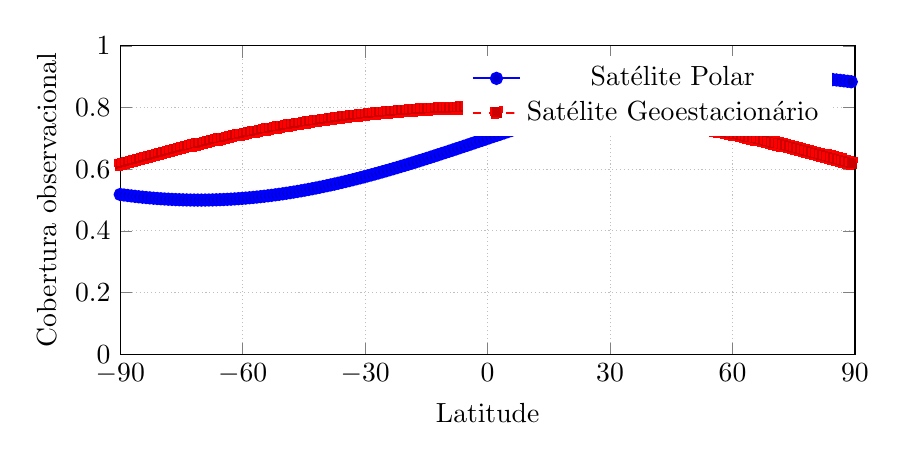
\begin{tikzpicture}
\begin{axis}[
  width=0.9\linewidth, height=5.5cm,
  xlabel={Latitude}, ylabel={Cobertura observacional},
  xmin=-90, xmax=90, ymin=0, ymax=1.0,
  grid=both, grid style={densely dotted},
  xtick={-90,-60,-30,0,30,60,90},
  legend style={at={(0.97,0.97)},anchor=north east,draw=none}
]
  \addplot+[smooth,thick,domain=-90:90,samples=200] {0.7+0.2*sin(deg(x/45))};
  \addplot+[smooth,thick,dashed,domain=-90:90,samples=200] {0.4+0.4*cos(deg(x/90))};
  \legend{Satélite Polar, Satélite Geoestacionário}
\end{axis}
\end{tikzpicture}
\caption{Cobertura observacional média por latitude. Nos trópicos, os satélites geoestacionários (como GOES-16) são essenciais para compensar a falta de sondagens.}
\label{fig:cobertura-tropicos}
\end{figure}

%---------------------------------------------------------
\section{O papel dos novos sensores e observações emergentes}
O avanço instrumental abre uma nova era para a assimilação:
\begin{itemize}
  \item \textbf{Satélites de nova geração:} GOES-R, MTG, METOP-SG e JPSS fornecem medições hiperespectrais e temporais de alta resolução;
  \item \textbf{Microssatélites e constelações:} missões CubeSat (TROPICS, CYGNSS) aumentam a densidade observacional nos trópicos;
  \item \textbf{Sensores de superfície inteligentes:} redes IoT meteorológicas e agrícolas permitem assimilação de dados locais em tempo real;
  \item \textbf{Radar de dupla polarização:} fornece observações tridimensionais de hidrometeoros e vento vertical;
  \item \textbf{GNSS-RO e interferometria:} melhoram o perfilamento da atmosfera em escala global.
\end{itemize}

Essas novas fontes de dados impõem desafios de calibração e controle de qualidade, mas ampliam consideravelmente o potencial preditivo dos modelos numéricos.

%---------------------------------------------------------
\section{Síntese e perspectivas}
O futuro da assimilação de dados caminha para sistemas:
\begin{itemize}
  \item \textbf{acoplados e multiescalares}, integrando componentes do Sistema Terrestre;
  \item \textbf{inteligentes}, com aprendizado adaptativo de erros e relações entre variáveis;
  \item \textbf{massivamente paralelos}, explorando arquiteturas de HPC e computação exascale;
  \item \textbf{autônomos}, capazes de operar continuamente com entrada de novos sensores.
\end{itemize}

A fronteira entre modelo e observação tende a desaparecer: cada modelo será, em essência, um assimilador dinâmico, ajustando-se permanentemente ao mundo real.
Essa visão coloca a assimilação de dados como um pilar central da ciência de previsão — o elo entre observação, teoria e simulação numérica.

% Fim do Capítulo 11
